\section{Vincoli d'integrità}
Nelle relazioni tra entità esistono diversi \textit{Vincoli d'integrità}. Di fondamentale importanza è il \textit{Vincolo di Cardinalità}.
\subsection{Vincolo di Cardinalità}
Il \textit{Vincolo di cardinalità} specifica il rapporto che esiste - in una data relazione - tra un intervallo minimo e massimo di istanze di un'entità e la relazione della stessa con un'altra entità.
\paragraph{Esempio.}
Abbiamo due entità \textit{impiegato} e \textit{città}, modellate in una relazione \textit{residenza}.
Dobbiamo indicare, nel diagramma \textit{ER} il vincolo di cardinalità:
\begin{itemize}
    \item lato \textit{impiegato}-\textit{residenza}, sappiamo che ad ogni istanza di impiegato possiamo associare una ed una sola abitazione di residenza. Perciò il nostro vincolo indicherà un intervallo di \textit{(1,1)} (\textit{da 1 a 1});
    \item lato \textit{città}-\textit{residenza}, invece, sappiamo che per ogni istanza di città possono esistere un numero variabile di abitazioni di residenza. Perciò il nostro vincolo indicherà, in questo caso, l'intervallo \textit{(0,N)}.
\end{itemize}
\begin{center}
    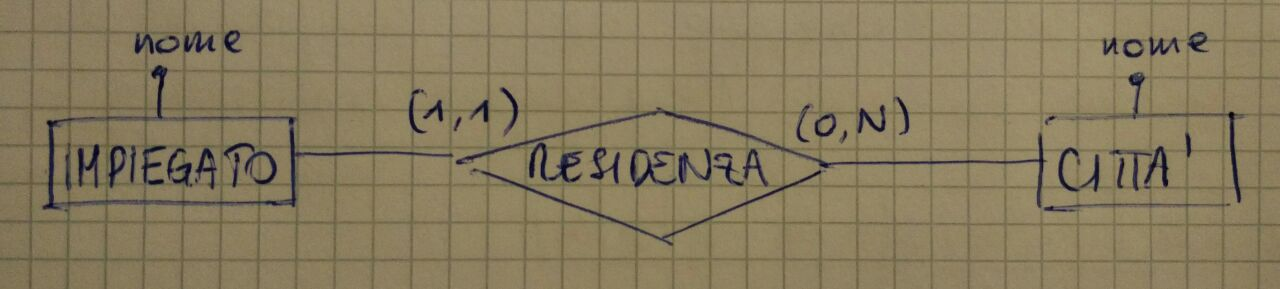
\includegraphics[width=.7\textwidth]{res/er-impiegato-citta.jpg} \hfill
\end{center}
\paragraph{NB.}
Un'entità può essere coinvolta in diverse relationships.
\newpage

\paragraph{Esercizio 1}
Dobbiamo modellare la relazione che gestisce i docenti in un ateneo. Sappiamo che ogni docente è determinato da:
\begin{itemize}
    \item nome e cognome;
    \item ruolo:
    \begin{itemize}
        \item RU (Ricercatore Universitario)
        \item PA (Professore Associato)
        \item PO (Professore Ordinario)
    \end{itemize}
    \item dipartimento.
\end{itemize}
Ogni dipartimento invece sarà determinato invece da:
\begin{itemize}
    \item direttore (istanza di docente)
    \item nome
\end{itemize}
Il risultato finale sarà il seguente:
\begin{center}
    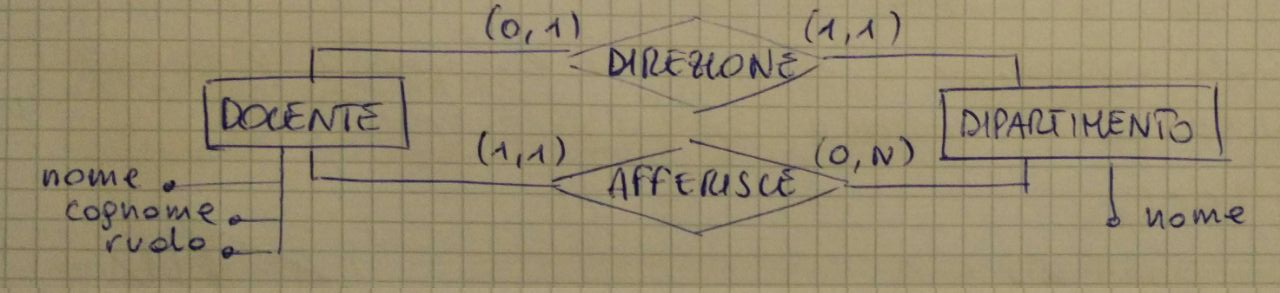
\includegraphics[width=.7\textwidth]{res/er-docente-dipartimento.jpg} \hfill
\end{center}
Lo schema delle entità quindi seguirà le seguenti tabelle: \\
\begin{minipage}[t]{0.5\textwidth}
    \captionof{table}{\textbf{Docente}}
    \begin{center}
        \begin{tabular}{|l|l|}
            \hline
            \textbf{Attributo} & \textbf{Dominio} \\ \hline
            nome        & stringa       \\ \hline
            cognome     & stringa       \\ \hline
            ruolo       & {RU,PA,PO}    \\ \hline
        \end{tabular}
    \end{center}
\end{minipage}
\begin{minipage}[t]{0.5\textwidth}
    \captionof{table}{\textbf{Dipartimento}}
    \begin{center}
        \begin{tabular}{|l|l|}
            \hline
            \textbf{Attributo} & \textbf{Dominio} \\ \hline
            nome        & stringa       \\ \hline
        \end{tabular}
    \end{center}
\end{minipage}

\paragraph{Esercizio 2}
Scrivere il diagramma \textit{ER} che modelli la seguente struttura:
\begin{itemize}
    \item impiegato: nome, cognome, data di nascita, stipendio, (unico) dipartimento, (più) progetti;
    \item dipartimento: nome, numero telefonico, data afferenza, (più) impiegati, (unico) direttore (istanza di impiegato);
    \item progetto aziendale: (più) impiegati, nome, budget.
\end{itemize}
\begin{center}
    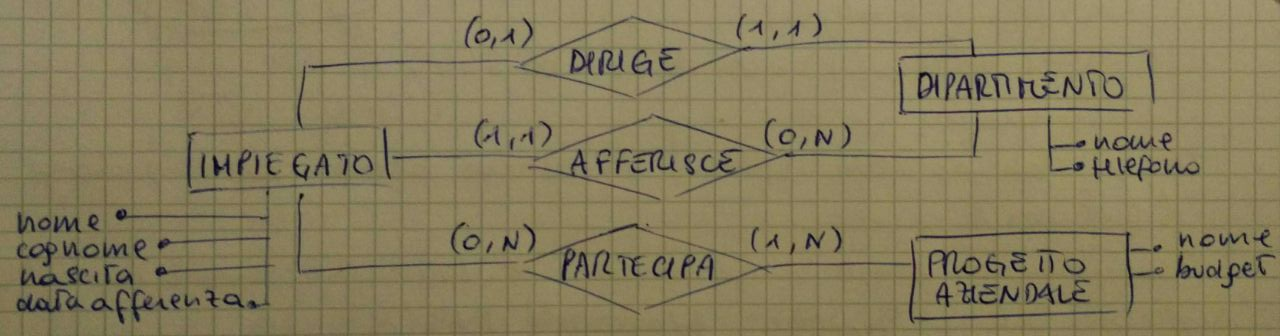
\includegraphics[width=.7\textwidth]{res/er-impiegato-dipartimento-progettoaziendale.jpg} \hfill
\end{center}

\section{Ruoli di Relationship}
Possiamo avere relationships che coinvolgono più volte una stessa entità. Da qui nasce il concetto di \textit{ruolo di relationship}, per cui a ciascuna relazione viene associato un nome di identificazione. \\
Per esempio, vogliamo collegare un'istanza di \textit{presidente} al suo \textit{predecessore} (istanza dello stesso \textit{presidente}):
\begin{center}
    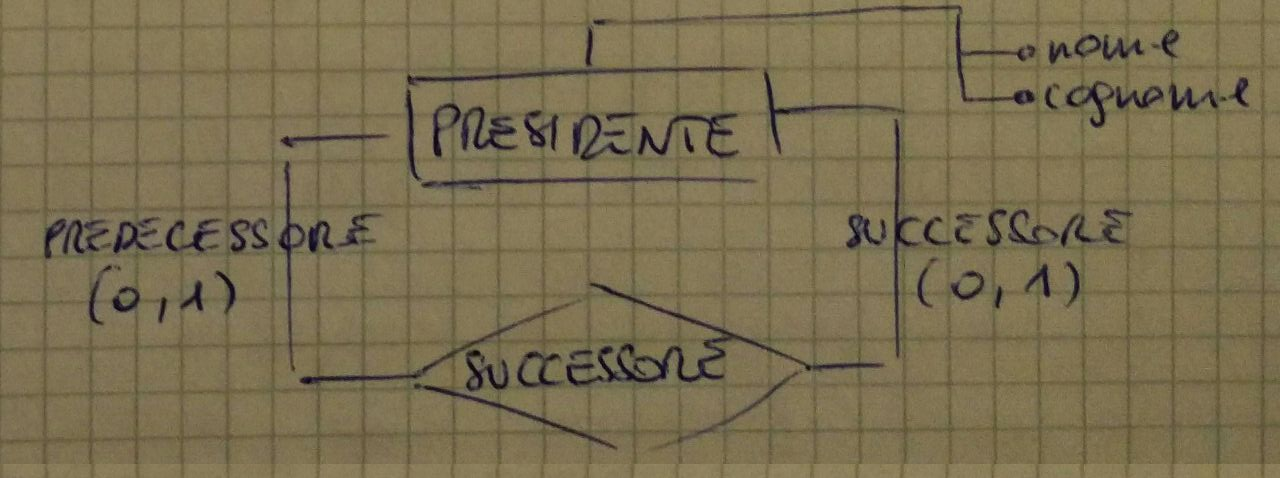
\includegraphics[width=.7\textwidth]{res/er-presidente.jpg} \hfill
\end{center}
Possiamo avere un numero variabile di ruoli per la stessa relazione, non limitandoli necessariamente a due.

\section{Attributi di Relationship}
Anche le relationship possono avere attributi, proprietà locali che associano a ciascuna relationship (o meglio, a ciascuna istanza di quella relationship) un valore di un certo dominio (tipo).
\begin{center}
    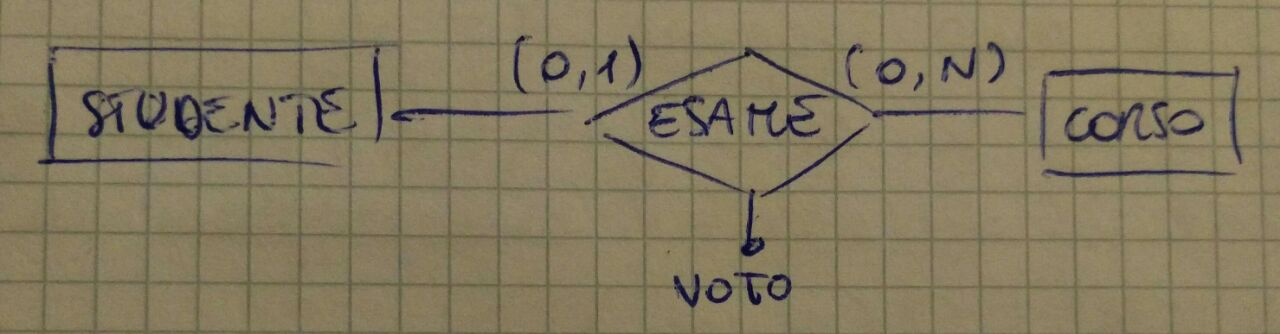
\includegraphics[width=.7\textwidth]{res/er-studente-corso.jpg} \hfill
\end{center}

\section{Relazioni \textit{IS-A} tra Entità}
Per il momento abbiamo lavorato su entità totalmente distinte tra loro. Esiste però il concetto di \textit{is-a}, che rappresenta il concetto di \textit{ereditarietà} per il linguaggio \textit{ER}. \\
Sostanzialmente, date due entità \textit{studente} e \textit{persona}, si dice che \textit{studente} è (\textit{is-a}) istanza di \textit{persona}, e quindi:
\begin{itemize}
    \item \textit{persona} rappresenta l'\textit{entità base};
    \item \textit{studente} rappresenta l\textit{entità derivata} (o \textit{figlia}, o \textit{sottoentità}).
\end{itemize}
A livello estensionale, in ogni momento ogni istanza di \textit{studente} deve essere un sottoinsieme delle istanze di \textit{persona}.
Se \textit{persona} ha l'attributo \textit{nome} e \textit{studente} l'attributo \textit{matricola}:
\begin{itemize}
    \item ogni \textit{persona} ha soltanto un \textit{nome};
    \item ogni \textit{studente} ha non solo un numero di \textit{matricola}, ma anche un \textit{nome}.
\end{itemize}
\begin{center}
    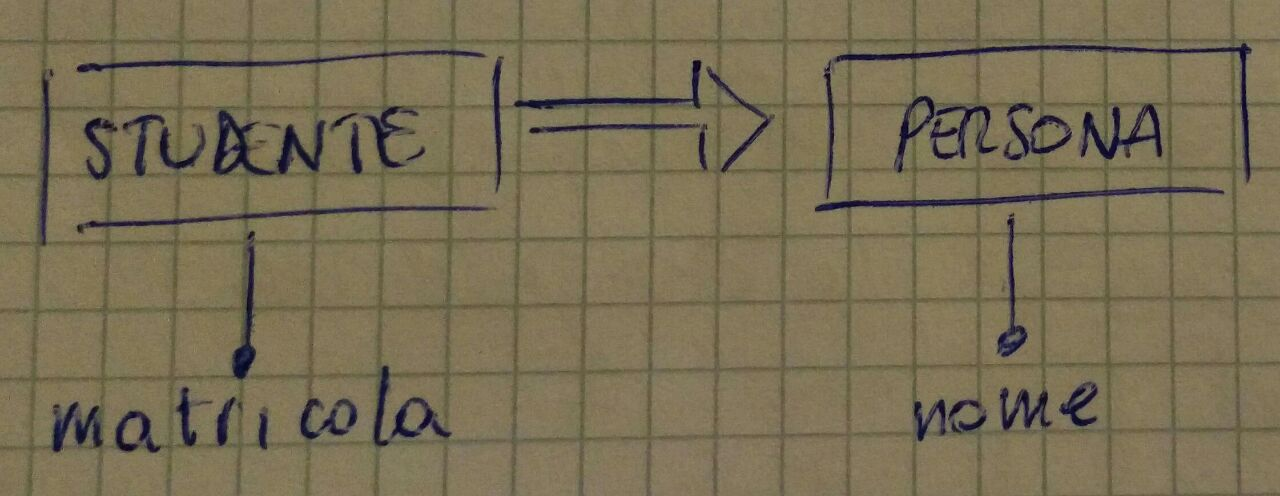
\includegraphics[width=.7\textwidth]{res/er-studente-persona.jpg} \hfill
\end{center}

\section{Transitività}
La \textit{transitività} rappresenta la ricorsione del concetto di \textit{is-a}, l'\textit{ereditarietà di ereditarietà}.
\begin{center}
    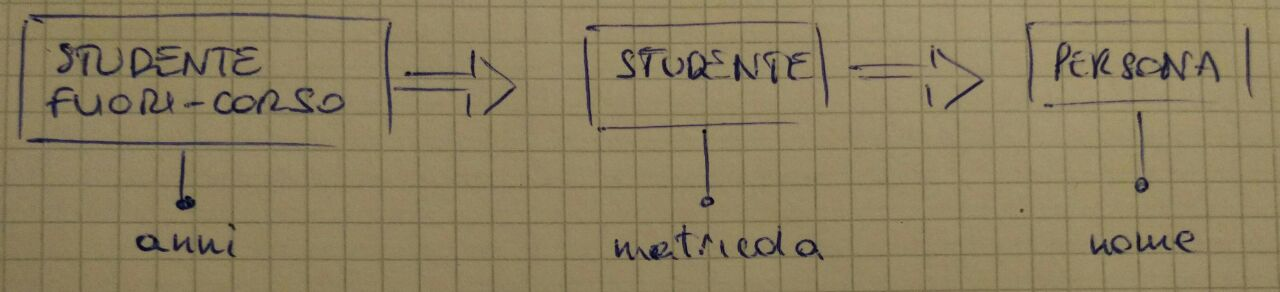
\includegraphics[width=.7\textwidth]{res/er-studentefuoricorso-studente-persona.jpg} \hfill
\end{center}

\section{Generalizzazione tra Entità}
La \textit{generalizzazzione} tra entità definisce una sorta di attributo di un'entità, definibile - distintamente - tramite l'uso di apposite altre entità.
\begin{center}
    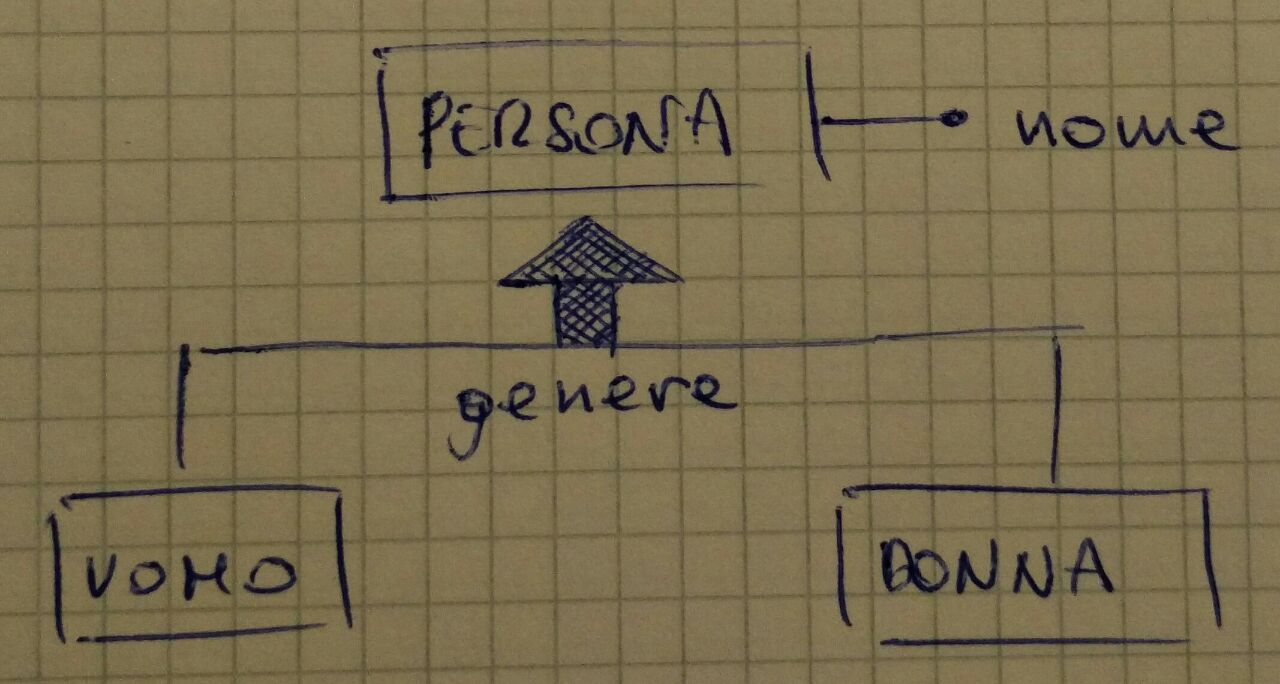
\includegraphics[width=.5\textwidth]{res/er-persona-uomo-donna.jpg} \hfill
\end{center}
Porta tre proprietà:
\begin{enumerate}
    \item \textbf{disgiunzione}: $uomo \neq donna$;
    \item \textbf{completezza}: ogni \textit{persona} è sempre o \textit{uomo} o \textit{donna};
    \item ogni \textit{uomo}/\textit{donna} è anche \textit{persona}.
\end{enumerate}
\paragraph{NB.}
Il linguaggio \textit{ER} permette l'ereditarietà multipla, ma non la generalizzazione multipla.

\section{IS-A tra Relationship}
\begin{center}
    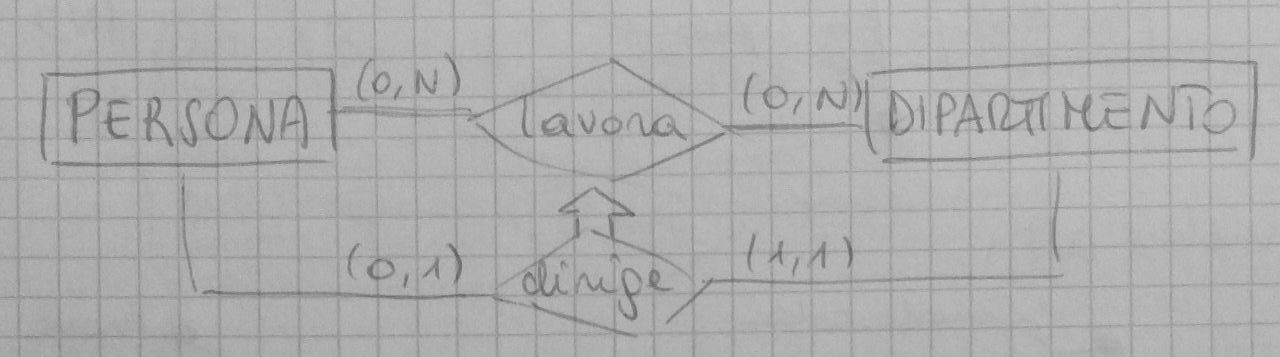
\includegraphics[width=.7\textwidth]{res/er-isa-relationship.jpg} \hfill
\end{center}
Realizzare IS-A tra relationship è possibile soltanto tra relazioni dello stesso tipo, dove per \textit{tipo} si intende il prodotto realizzato tramite l'incrocio delle entità che queste legano. \\
In questo sono considerate entità confrontabili e analoghe le IS-A:
\begin{center}
    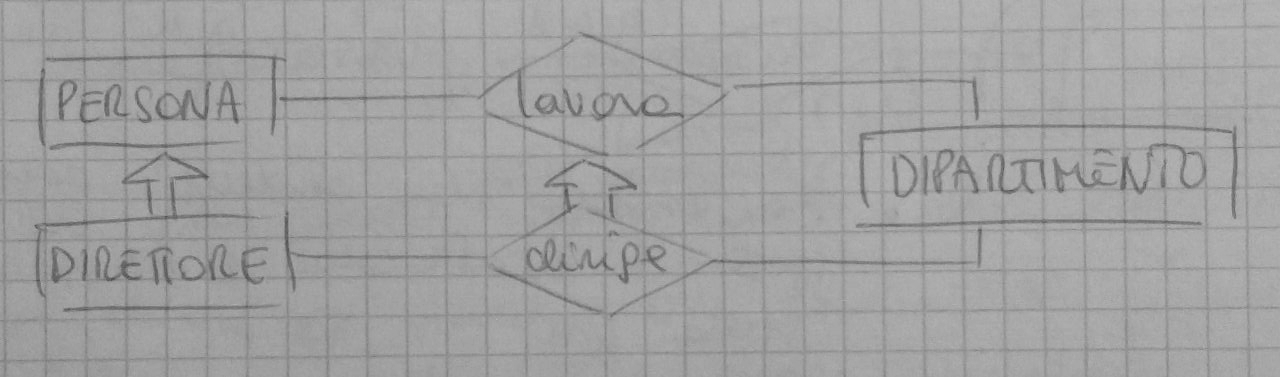
\includegraphics[width=.7\textwidth]{res/er-isa-relationship-isa-entities.jpg} \hfill
\end{center}
In sostanza, le condizioni che devono essere rispettate perché una relationship $rel_{1}$ sia una IS-A di una relationship $rel_{1}$ sono le seguenti:
\begin{enumerate}
    \item $rel_{1}$ e $rel_{2}$ devono avere pari arità;
    \item $rel_{1}$ e $rel_{2}$ devono avere gli stessi ruoli;
    \item per ciascun ruolo comune alle due relationship, le entità corrispondenti a questo ruolo nelle due relationship devono essere necessariamente, a loro volta, istanze della stessa entità o una l'IS-A dell'altra;
    \item il valore del vincolo di cardinalità proposto da $rel_{2}$ deve essere compatibile con quello espresso da $rel_{1}$, e/o viceversa.
\end{enumerate}

\section{Vincoli di Cardinalità su Attributi}
È possibile applicare vincoli di cardinalità anche su attributi di una entità/relationship. Possono quindi rappresentare:
\begin{itemize}
    \item opzionalità;
    \item valori multipli.
\end{itemize}
\begin{center}
    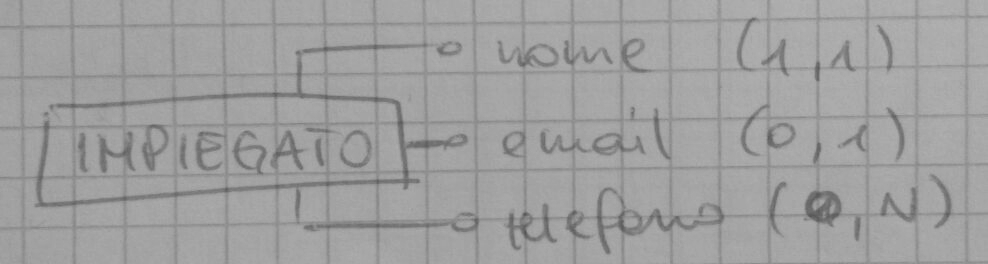
\includegraphics[width=.7\textwidth]{res/er-cardinalita-attrs.jpg} \hfill
\end{center}

\section{Vincoli di Identificazione su Entità}
Un identificatore per un entità è un insieme di attributi e/o ruoli di relationship, tale che non esistono due istanze di questa entità che abbiano stesso valore su quell'insieme di attributi.
\begin{center}
    \textbf{Identificazione su un solo attributo} \\
    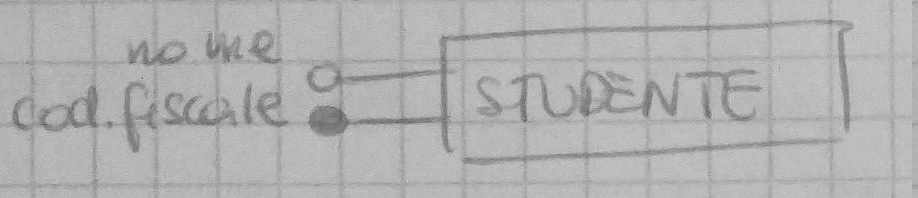
\includegraphics[width=.7\textwidth]{res/er-identificazione-1.jpg} \\
    \textbf{Identificazione su un insieme di attributi} \\
    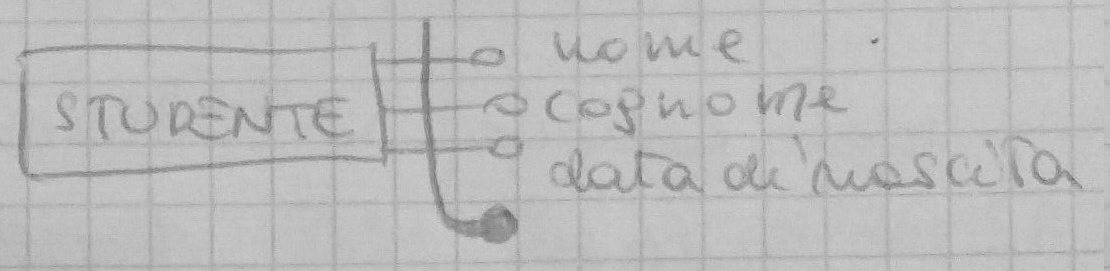
\includegraphics[width=.7\textwidth]{res/er-identificazione-2.jpg} \\
    \textbf{Identificazione su un insieme di attributi e ruoli} \\
    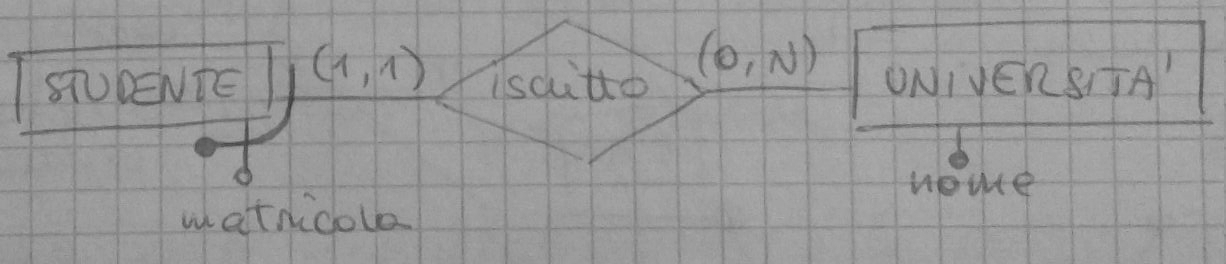
\includegraphics[width=.7\textwidth]{res/er-identificazione-3.jpg} \\
    \textbf{Identificazione su un insieme di ruoli} \\
    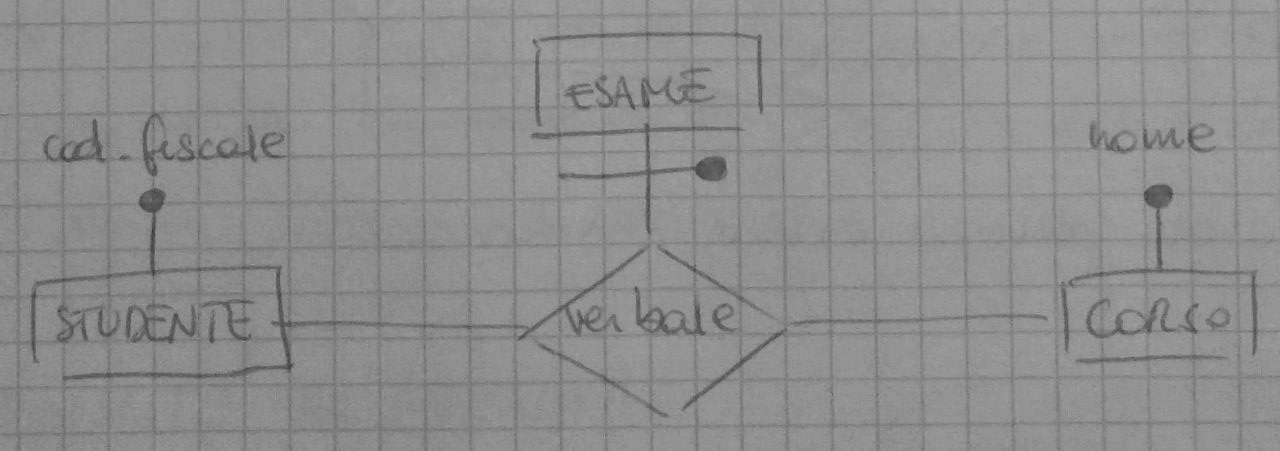
\includegraphics[width=.7\textwidth]{res/er-identificazione-4.jpg} \\
\end{center}
È di fondamentale importanza che ciascun identificatore sia il più minimale possibile.

\section{Vincoli Esterni}
Vincoli non esprimibili direttamente in diagrammi \textit{ER}, che prendono il nome di \textit{business rules}, che sono sostanzialmente le regole di funzionamento del sistema. Sono di norma specificati nel \textit{dizionario dei dati}, attraverso l'uso della logica matematica.